\documentclass[a4paper,10pt]{article}
\usepackage{url}
\usepackage{hyperref}
\usepackage[shadow]{todonotes}


%opening
\title{Find the Treasure!\\Building a Multiplayer Javascript Game Using Cloud Services\footnote{The game and code are available on \url{http://student.science.uva.nl/\~mmvdv/findthetreasure/}}}

\author{Maarten van der Velden\\maarten.vandervelden@student.uva.nl\\Student ID: 5743087}
\date{\today}

\begin{document}

\maketitle

\section{Introduction} % (fold)
\label{sec:introduction}
For the Project of the Game Programming course in the Master AI, I decided to  try and make a multiplayer game that does not need to run a dedicated server, but relies on cloud services only. It was initially influenced by a project I did for a course in Information Visualization, where I used Google Street View\footnote{\url{http://maps.google.com/help/maps/streetview/}} as a means of visualizing spatial data. The idea to use Google Street View for making a game was not a big step from there. As the most advanced API of Google Maps \footnote{\url{https://developers.google.com/maps/documentation/javascript/}} is written in Javascript, this was the obvious choice as a programming language. This enabled me to make the game browser-based, and readily available to publish
online. During the project I realized more and more that with today's internet speeds and online services, I would not need to host the game on an online server. I use a free web socket server (EasyWebSocket\footnote{ \url{http://easywebsocket.org/}}) to let players communicate. At client side, the game also takes relatively little processing power, because most of the rendering is done online by Google Maps.

From a gameplay perspective, the goal of the game is to find a treasure that is hidden somewhere in the world, by means of Google Street View. In this way, you make a  virtual quest from your original location in search of the treasure. Your guides to this are limited, as you only get rough hints about how you are doing. In the multiplayer game, you play live against an opponent, and you try to reach the other's starting location as quickly as possible in order to capture your opponent's flag. The game has a number of settings and extras to make things interesting, such as playing at your current location. There are many possibilities for expansion too.

All in all I think I have made a game that, although the concept is simple, is very fun to play, has lots of possibilities for extension, and complies very much with recent trends, mostly the various web-based apps that use cloud computing that appear everywhere. The game is not yet ready for publication, mostly because little effort is put in the design, and little tests are done on the game experience by real users. It can be seen as a proof of concept that the possibilities of making a javascript game using web services like Google Maps are quite big, and with as little experience as I have in game making and webdevelopment, it is possible to make a fun online multiplayer game.

In this report I explain how the game was made. First I will tell something about the different building blocks of the game. In section 3 I will explain how the game came to be designed as it is. In section 4 I will discuss the game modes and gameplay, including both possible extensions and things that would need to be fixed at least for a release on larger scale. In the last section draw a short conclusion.

% section Introduction (end)
\section{Building Blocks} % (fold)
\label{sec:building_blocks}
The game is basically an HTML webpage, dynamically build using Javascript.
I use three web services to make this game work, the Google Maps API, EasyWebSockets, and MooTools. The first one is a very extensive API to make
a personal experience of Google Maps. Next to fully customizable Google Map windows and adding layers to these, it is possible to do path planning, do
geographical calculations and use Street View. The Street View functionality forms the basis of the game, while I use some other features too for the various game elements.

EasyWebSockets provides, just like the name suggests, a very basic and easy web socket service, hosted free. Using this service, clients on the same url can broadcast messages to all other visitors asynchronously. This is used to communicate live game data in multiplayer games, mostly the players's location and progress towards their goal.

MooTools\footnote{\url{http://mootools.net/}} is a Javascript toolbox to make it easy to dynamically use HTML webpages. I use it for all kinds of behind-the-screens work, mostly regarding the visualization on the webpage, such as showing, hiding and changing of interface objects, and using the game menu.

With these three web services, I started the implementation of the game.

I implemented and tested this game using the Google Chrome browser on Mac OSX Lion. I did not really test it in other browsers, so I cannot guarantee its working with other system configurations at the moment.

% section building_blocks (end)

\section{Development} % (fold)
\label{sec:Development}
The game was developed quite organically. I started out with the idea of making a game to find `Easter Eggs' in Google Street View, after I discovered the Maps API supplied tools to make users visit a Street View page without the possibility of exiting to a Map view. Furthermore, I learned that it was possible to navigate Street View using the keyboard's arrow keys, creating a more game-like experience than clicking around.

The basic idea was to be put at a random location in Street View, and there would be an Easter egg hidden somewhere else. The only clue the player would get is a very vague `Warmer' or `Cooler' (heat-based hints), indicating that the player would get closer, respectively further away from the Easter egg. This is also the way my parents would give hint when I was looking for Easter eggs when I was young.

After having implemented this basic idea, and showing it to some friends, I realized that finding the goal was rather hard with only these limited hints. This was mostly because the heat-based hints were given based on the Euclidean distance from the player to the goal, \emph{as the bird flies}. In a town like Amsterdam, where most streets are twisted and have turns everywhere, this often caused seemingly contradictory hints, and sometimes there is no road in the direction you should want to go. (Or there is a road, but it has no Street View because the Google cars didn't visit it.)

Also, because the player didn't get any hints on how much `hotter' or `cooler' he was getting, it might well be that he ended up going almost perpendicular to the optimal direction, causing the player to get in a street parallel to the Easter egg.

Keeping these experiences in mind, I decided to extend the game. I added more information sources, like a map of the area around the player, a bar that keeps track of your general progress and a compass that points towards the eggs. Also, because it is not Easter the whole year, I replaced the Easter eggs with treasures.

Furthermore I thought an online game cannot go without a multiplayer function. Because I have only very little experience in network programming and database management, I looked for a solution as light weight as possible. I first thought of using the Facebook API for user management and playing with friends, but because I would have to do the user management myself, using the Google App Engine or something similar, I thought, for the moment it would be sufficient to show that multiplayer would work at all, and I crossed the EasyWebSockets website\footnote{\url{http://easywebsocket.org/}}.

I chose to keep the multiplayer game very simple for the moment, and make it a two player capture the flag game, where the starting point of player A is the goal of player B. So you don't only have to find the treasure, but your opponent is doing the same thing at the same time, in the opposite direction. I thought that in this way, the benefit of a multiplayer version would be greatest. It is real-time, you can see your opponent's progress alongside yours, and view his location on the map and in Street View itself, if you're close enough to each other. Being close to each other is stimulated by having the goals in the opposite direction. Another option would have been to make it a race, with the same start and finish positions.

I did not pay much attention to the interface before starting the game. The welcoming screen and menu are rather crudely designed, and as the website has no user management system, I cannot let player choose their opponent from the game. To enable this, I make a random url for each multi-player game. The first player who visits after the player who \emph{hosts} the game, will play with the settings the host shows. The host, who makes the game, should send a message with the url to the other player using a channel outside the game, such as a mail, messaging, or chat system. The main downside of this is that the game host cannot leave or reload the game site before starting the game, because some game settings are stored temporarily in the host's web page only.

% Continue explaining gam modes and the game screen
\section{Gameplay} % (fold)
\label{sec:gameplay}
\begin{figure}[hbt]
    \centering
    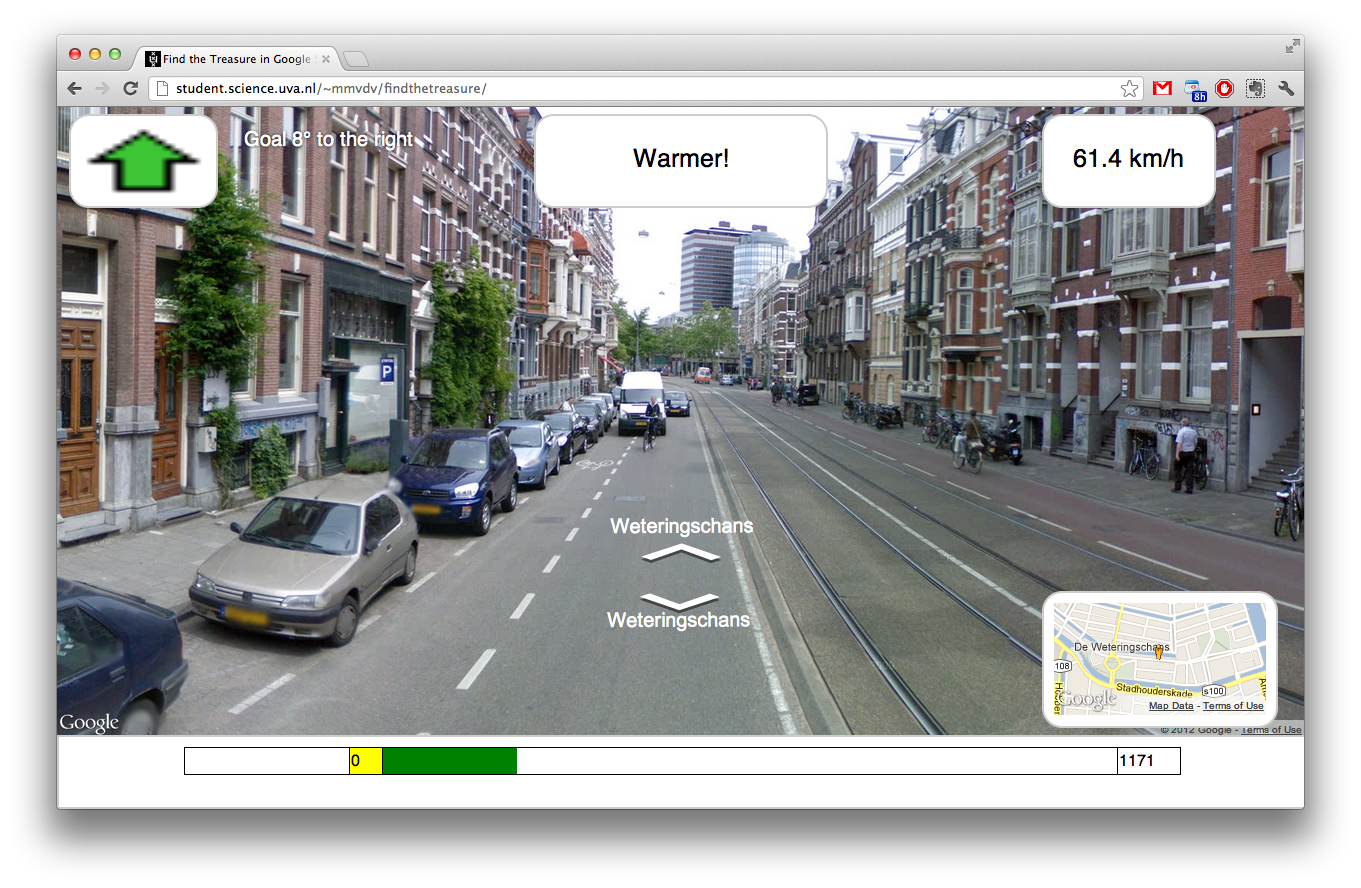
\includegraphics[width=\textwidth]{screenshot}
    \caption{Screen shot of the game. The top center box is the Heat-O-Meter, on the bottom is the Progress Bar, the top left gives the compass, and on the lower right is the map. On the top right is an indication of the current speed, for fun.}
\end{figure}

The main goal of each game mode is to reach the goal, a treasure, by `walking' through Google Street View. There are four clues that help the player with this:
\begin{description}
    \item[Heat-O-Meter] The main clue of the game, displays wether the player is closer (warmer) or further off (cooler) of the treasure than before his last move.
    \item[Progress Bar] A bar that shows the player's progress from his original position towards the treasure. The progress is measured as a bird flies, without regarding the road map nor Street View accessibility. In a multi-player setting, the opponents progress is shown as well, which gives an easy clues who is closer to the goal, and creating a sense of competitiveness.
    \item[Compass] A compass that always points in the general direction of the goal (disregarding streets). The Heat-O-Meter might show the player is going in the right direction, but he might be going parallel alongside the goal. The compass indicates when this is the case.
    \item[Map] The map is centered on the user, and shows the treasure if it is within the area. It gives information on the street profile of the area, making it easier for the player to find a route towards the goal. In multiplayer, the opponent is shown on the map too, too enhance the feeling of real-time playing together.
\end{description}

Depending on the difficulty setting, these clues might or might not be available. There are three difficulty settings:

\begin{tabular}{r||c|c|c|c}
    Difficulty & Heat-O-Meter & Progress Bar & Compass & Map \\
    \hline \hline
    Easy    & x & x & x & x \\
    Normal  & x & x & x & \\
    Original& x & x &   &
\end{tabular}\\
There are 3 game modes available currently:
\begin{description}
    \item[Tutorial] In this mode, the controls and elements of the game are explained in three short `levels'. The user is also being prepared for the quirks that might appear in Street View, such as streets missing Street View coverage and therefore not navigable, missing links between two Street View panoramas that are only navigable by clicking using the mouse, and Google not regarding height of panoramas very well which may cause users to end up in a tunnel suddenly.
    \item[Single Player Free Play] The basic game mode, where the player can select where he wants to play, what difficulty he wants, and at what distance the treasure must be. An option to play at the player's real geolocation is available here.
    \item[2-Player Capture the Flag] The multi-player mode, where the host player can setup a game like a free playing game, after which a link is provided that can be said to the opponent, after which a game starts where the treasure of the host player is a flag hidden at the start location of the client player, and vice versa.
\end{description}
A number of possible future game modes will be given in the next subsection. 

While playing the game, the user sees a Street View panorama, with the cue elements (Heat-O-Meter, Progress Bar, Compass, Map) around it. Navigation is identical as usual in Google Street View. This means there are three ways of navigating: 
\begin{enumerate}
    \item The user can click the arrows displayed in the panorama that indicate the possible ways to navigate from the current panorama;
    \item When moving around the mouse over the panorama a circle lights up at times, usually on roads, indicating that a click will result in moving to a panorama near that location.
    \item If the panorama has focus, the keyboard's arrow keys can be used to navigate through Street View, where the up and down keys cause going to the adjacent panoramas in the direction closest to straight ahead and straight back respectively. The right and left arrow keys cause the player to pan the panorama in that direction.
\end{enumerate}
Furthermore, dragging with the mouse can also be used for panning.

When the player comes within reach of the goal, it will be visible as a moving image in Street View. When the player is within 30 meters, the game is ended and the user has the opportunity to restart. In multiplayer, when the other player reaches the goal first, the player is notified that he is lost. The game is over in this case too. Furthermore, in multiplayer the players can see each other in Street View when close enough to each other, as a green peg man. This serves the feeling of real-time competition. All images in Street View might seem to be visible `through buildings' because the icon renderer of Street View does not take the image on which the icons are projected into account.

\subsection{Other Elements} % (fold)
\label{sub:other_elements}

Next to the functionality currently implemented, there are lots of other possible game modes and functionality to be thought of.

A very obvious game mode would be to add a Campaign mode, where multiple levels of increasing difficulty should be played. This might be a nice way to make a show case of interesting spots to see on Street View, or strange places that apparently can be visited. It might be nice to add a level where a very long distance trip should be made.

Furthermore, more multiplayer modes could be made, for example a race mode from the same origin to the same goal. This could also be more than 2-player, for there is no real limit to the amount of players playing concurrently.

In multiplayer mode, it might be nice to be possible to play against the computer, by making a bots that can play the game. The most simple would be a bot that always takes the direction that minimizes its distance to the goal, a more sophisticated one could actually keep in mind its history and do some kind of depth-first search. A probably hard-to-beat agent would be one that uses Googles path finding function to find an efficient route and walk this.

It would also be possible to make some kind of multiplayer shooter-style game, though it should be kept in mind that the communication protocol probably is not fast enough to shoot each other real-time. Furthermore, Street View provides no kind of collision detection. It could be possible however to play a kind of tag or catch by letting players work in teams and try to capture each other by cutting of all routes of escape. It would also be possible to make a MMO of the game, by letting everyone walk around in the same panorama, being able to see each other. A game element should be designed for such a game mode too.

Adding power-ups etcetera to Street View would also be an option, these might for example be a possibility to get more help to find the treasure such as  getting a hint for the direction, showing the route, or have a sneak peek at it, or a teleport to a new location. These could be in-game pick-ups, or benefits that can be earned. For multiplayer, these power-ups could be road blocks, mines, random teleports, or any other means to keep back the opponent. It might even be possible to let people buy in-game assets like these.

Storing user progress and achievements would be a good addition too. This enables the game to make players achieve certain things before making other functionality available, which keeps players attached to the game. It would also be nice if players could compare each others scores and achievements. For this a scoring system and achievement system should be added too.

All in all, the game has more than enough possibilities for expansion to make it more attractive and possibly addictive to users. Possibly, adding all these features would be too much, and it would be better to focus on certain game modes to avoid choice stress for players.

% subsection missing_elements (end)
\subsection{Missing Functionality} % (fold)
\label{sub:missing_functionality}
Currently, the game is in quite an early stage of development. The gameplay as explained all works, but is not fully tested on all kinds of situations. The most striking improvements would be to make a good design of the user interface and the in-game elements (right now, the treasures are still represented by Easter eggs and bunnies), and to improve the multiplayer functionality, by not having to send the game url externally. For the latter, I have considered using for example Facebook account management. Facebook has a good API, which could allow users to see who of their friends are logged into the game currently, and invite them for a game.

Furthermore, it would be necessary to make the game compliant with other browsers next to Chrome, because you do not want to force the player into a certain kind of player. A mobile version would be interesting too. Because it is Javascript based, it would be possible to run it on iPhones. But the functionality of Street View on mobile devices should be tested first.

Another fix that would be necessary before seriously releasing this game would be to remove some quirky events happening when playing the game, like the compass sometimes losing its sense of direction, the repeated finished message when a player decides to play on after the game-over message, and prohibiting this continuation of play at all. Extensive tests of the game will probably reveal many more bugs like these.

% subsection missing_functionality (end)
% section gameplay (end)

\section{Conclusion} % (fold)
\label{sub:conclusion}
All in all, the game show a working use case for a cloud-based game, based on Javascript. It is clear that this is more a proof of concept than a game ready for release. The only part not within control of the developer is the efficiency of the Street View interface. Unfortunately loading times of the images can be fairly long, hampering the game experience. Using a commercial, paid, subscription to the Google API could partly solve this, although games with this setup will always have to cope with the probability of a user having a slow internet connection. This is the main disadvantage of working in javascript and using cloud-based services, next to their limited customizability. It would have been nice to have some more control over the look and feel of Street View, but this is not possible from the API. The advantage on the other hand is the low processor cost at the client side and no real need for a game server.

Although the game is still a concept, it is also a work in progress, as I am planning to expand it, give it a better design and let people play it for real. There might be some improvements visible within a few months from now.
% subsection conclusion (end)
% section discussion (end)

\bibliographystyle{plain}
\bibliography{ref}
\end{document}